\clearpage\secrel{Managed compilation}\label{manacomp}\secdown

\noindent
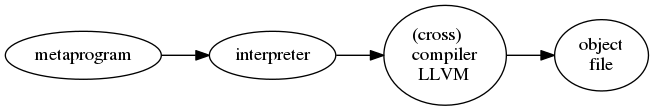
\includegraphics[width=\textwidth]{img/dynacomp.png}

\term{Metacircular managed compiler}

\noindent
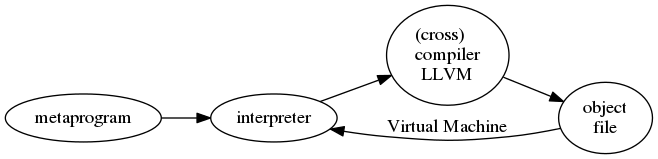
\includegraphics[width=\textwidth]{img/circomp.png}

\noindent
\term{Managed compilation} is \emph{compilation} by a compiler is
\emph{driven by meta\-program}. Classic compilers work in batch mode only: you
put a program for a target system, and get resulting executable code in batch.
Managed compilation extend your abilities to control compilation process in a
very fine grain, much more than macro\note{not available in many languages}.

\bigskip\noindent
\textcolor{red}{The price of power is complexity}: you must write full sized
\term{metaprogram} \emph{builds target code via calls to the compiler
framework}. This complexity can be amortized by using meta-libraries and OOP let
you use helpers and inheritable application templates.

\clearpage\noindent
You can use \term{static managed (cross)compilation} into executable object
files, if you need code for some embedded system, small executable files or
security hardened software system with unmodifiable code.

\bigskip\noindent
But the coolest method for ordinary large computers is running \term{dynamic
compilation} in a runtime, building machine code into RAM (some sort of managed
JIT on steroids). Dynamic compilation allows using \term{flex programming} based
on \emph{self-modifiable programs and nonsequential computation (hyper)graphs}.

\secrel{Metaprogramming (embedded \purec\ backend)}\secdown

\begin{framed}
\emph{Metaprogramming is} complex thing by design\ --- it is much simpler to
write \textit{single} program by hands, then \emph{write program that writes
program}.
\end{framed}

% \bigskip
\noindent
Metaprogramming is cool technique if your job is making a lot of typical
applications shares common code parts. So if you can distinguish a lot of
template-like code in your sources, you need a language with metaprogramming
capabilities. And it is not about macro\ --- \emph{you must have full scripting
at compile time} and access to your program code in the source code,
intermediate program representation, compiler structures and control on
compiling process itself.

\begin{framed}\noindent
If you are limited by some corporate rules, meta can let you generate program
source in pure C using \emph{\py} (or anything else) as the \emph{macro
language}.
\end{framed}

\noindent
Here you will be faced with complexity problem: metaprogramming is complex by
design, and the only way to hide this complexity\ --- use libraries and OOP, and
be ready for unavoidable complexity when you start.

\clearpage\secrel{Hello meta}

You already know this beast\ \ref{Object}:
\begin{lstlisting}[language=Python]
class Object():
	def __init__(self,V):
		self.value = V ; self.attr={} ; self.nest = []
	def __lshift__(self,V): return self.push(V)
	def push(self,o):
		self.nest.append(o) ; return self
	def __setitem__(self,K,V):
		self.attr[K] = V ; return self
	def __getitem__(self,K):
		return self.attr[K]
\end{lstlisting}
\clearpage\noindent
Dump object:
\begin{lstlisting}[language=Python]
	def __repr__(self): return self.dump()
    def head(self,prefix=''):
        return '%s<%s:%s>'%(prefix,self.__class__.__name__.lower(),self.value)
    def pad(self,N): return '\n'+'\t'*N
    def dump(self,depth=0):
        S = self.pad(depth)+ self.head()
        for i in self.attr:
            S += self.pad(depth+1) + self.attr[i].head(prefix='%s = '%i)
        for j in self.nest:
            S += j.dump(depth+1)
        return S
\end{lstlisting}
And here we are interested in metaprogramming:
\begin{lstlisting}[language=Python]
    def cpp(self): return '/* %s */'%self.head()
\end{lstlisting}

\secup


\clearpage\secrel{lol.VM in \py\ (LLVM backend)}\label{llvmpy}\secdown

For taking the first impression of pure managed compilation let's play with
\py\ only and LLVM compiler framework. The full source code you can found in
\href{https://github.com/ponyatov/o/blob/master/lol.py}{lol.py}.

\begin{lstlisting}
$ sudo apt install llvm
$ sudo pip install llvmlite
\end{lstlisting}

\noindent
If you are not friendly with bare LLVM, you can use online translator 
\url{http://ellcc.org/demo/index.cgi}\ lets you convert C/\cpp\ code into
LLVM assembly. And also you will need some entry tutorial on LLVM class model
itself you can find in \cite{llvmcore}. For simplicity, we'll use
\verb|llvmlite| binding to \py, and use some metaprogramming.

\pg
First, we can create only empty LLVM module:
\begin{lstlisting}[language=Python]
import llvmlite.ir as ir
# lol: Virtual FORTH Machine (LLVM portable)
module = ir.Module('lol')
print module
\end{lstlisting}
\begin{lstlisting}
; ModuleID = "lol"
target triple = "unknown-unknown-unknown"
target datalayout = ""
\end{lstlisting}

\secup

\secup
